\chapter{User Studies} \label{chapter:evaluation}
In the user study 1, we conducted an absolute detection threshold (ADT) study and a discrimination threshold (JND) study to investigate how users perceive normal force stimuli provided by FacePush. Additionally, we collected users' subjective ratings of their comfort with respect to the normal force feedback. Based on the results of user study 1, we determined the magnitude of normal force for the boxing application and ran an experience study using the boxing scenario.


\section{User Study 1: Psychophysics of FacePush}

\subsection{Absolute Detection Threshold (ADT) }
To determine the minimum normal force that is provided by FacePush that users can perceive, we conducted a standard two-down, one-up staircase study \cite{Lynette2012, Leek2001}. In each trial, both torque generators started rotating from their neutral state to a specific angle simultaneously. When the torque generators achieve the target angle, they maintain exertion of normal force on the face for a brief duration then return to their neutral state. The entire trial process is 4 seconds and the interval between two consecutive trials lasts 5 seconds. The experiment starts finding threshold from the high degree (150 degrees from the neutral state) to the absolute detection threshold. When participants perceive the stimulus twice consecutively, the target degree of the torque generators is decreased by a step size. Otherwise, the target angle increases if the stimulus is not felt at least once. The step size is 12 degrees and it is divided by two for every eight trials. The average of the last five trials performed are taken as the threshold estimate. These values were determined from a pilot study in which participants needed to complete 24 trials for three reversals. Each participant presses the play button when they are ready, but only once per trial, and responds with an answer of either “Felt” or “Not Felt” after each stimulus. For each trial, the participant's response was recorded and the corresponding angle of the torque generators. Each participant performed 72 trials in total and the entire procedure took approximately one hour to complete. During this study, the participant wore earphones with pink noise. Participants received a small gratuity as compensation for their time. 

\subsection{Results }
9 participants (4 females and 5 males, aged 22-26, mean age = 23.8) were recruited from our institution. The mean threshold estimate was 2.694 kilopascal (kPa) (95\% CI [2.558, 2.83]) which indicates that both torque generators must generate at least 2.694 kPa, which rotate 86 degrees from their neutral state such that a participant begins to feel the pressure on their face.

\subsection{Discrimination Threshold (JND) }
We are also interested in how users can distinguish a normal force stimulus exerted by FacePush. Hence, we conducted a just-noticeable difference (JND) study using the method of constant stimuli. Each participant had to respond \textit{same} or \textit{different} for each stimulus pair and each pair consisted of a base load and an offset load value. The torque generators can only rotate from 0 to 170 degrees and must rotate 86 degrees from their neutral state to reach the minimum detectable threshold. Thus the range in JND study is restricted to between 85 to 170 degrees from the neutral state of the torque generators. We use four base pressures (2.575, 2.700, 2.950, 3.450 kPa) and four offsets pressures ($\Delta$P) (0, 0.125, 0.250, 0.500 kPa) providing 16 different conditions. The base offsets increase exponentially in keeping with the JND standard. The order of conditions within the stimuli pairs is randomized and each participant must repeat two reversals, resulting in 32 trials in total. The interval, between the first stimulus and the second, is 5 seconds. After the first stimulus is given, FacePush returns to its neutral state and waits for 3 seconds then begins the second stimulus. The entire procedure during this study took about 20 minutes to complete and participants wore earphones with pink noise throughout the duration of the study. The same group of 9 participants (4 females and 5 males, aged 22-26, mean age = 23.8) that took part in our ADT study took part in this study several days later.

\subsection{Results }

\begin{figure}[h]
    \begin{center}
        \begin{tabular}{@{\hspace{0.1cm}}c}
            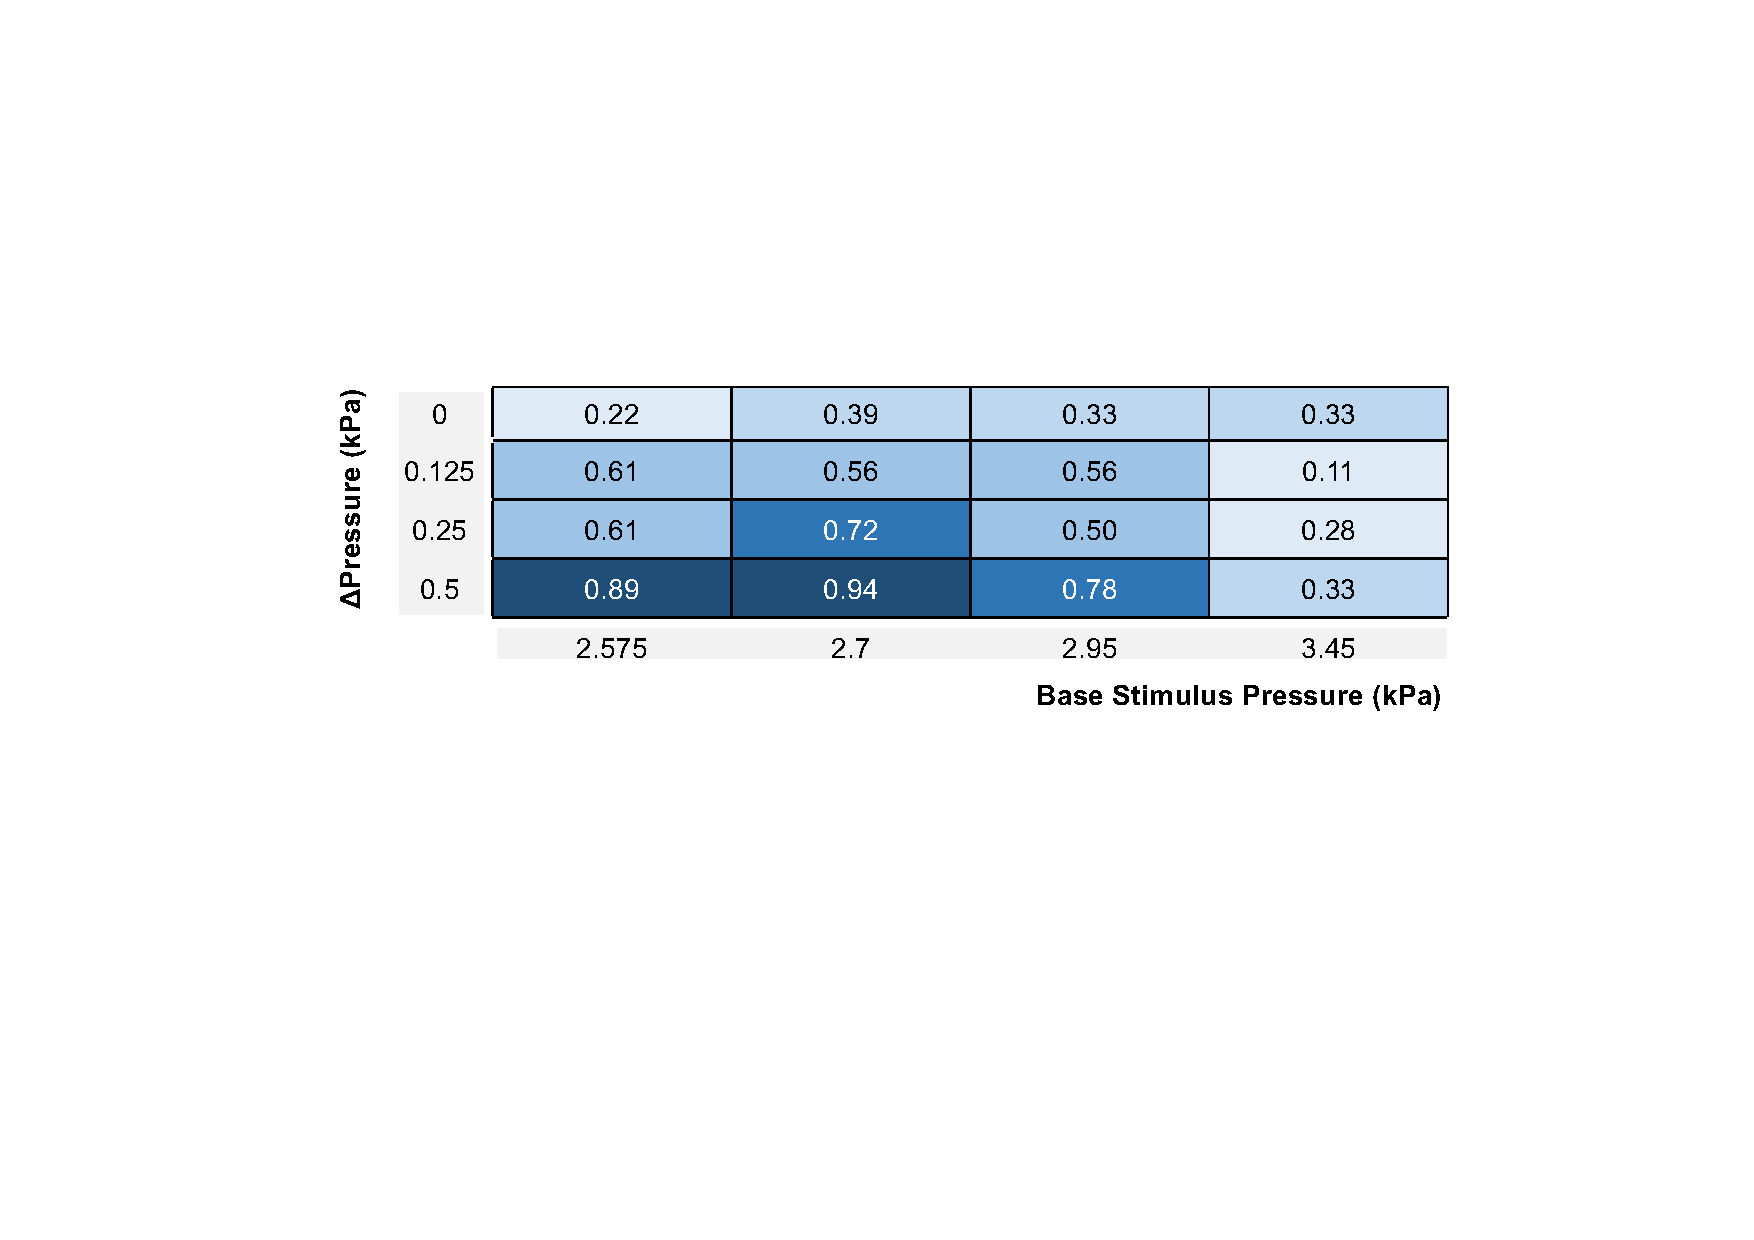
\includegraphics[width=1\linewidth]{figures/jnd}
        \end{tabular}
        \caption{Table shows the percentage of responses that judged the two stimuli as different. As baseload increases, offset needs to be higher.}
        \label{fig:jnd}
    \end{center}
\end{figure}

We define the JND as the pressure difference where 75\% of the users were able to distinguish two stimuli apart. By picking a 25\% error level, we obtained the difference where we can assume participants only confuse two different kinds of stimulus in 25\% of instances. The percentage of users who felt that a pair of stimuli are different is aggregated as a score for each base/offset pair (Figure \ref{fig:jnd}). The base rate, 2.575 and 2.700, need a $\Delta$P of 0.5 kPa so that the user can distinguish two stimuli. The other two base pressures, 2.950 and 3.450 did not perform well. We consider that these two base rates may need a greater $\Delta$P. However, not only adding more $\Delta$P for perceiving a difference from 3.450 kPa already exceeds the available range of FacePush, strong force may cause some concern in regard to comfort. Hence we selected 2.575 and 2.7 kPa as the base pressure for the comfort experiment. We determined the 75\% JND for each base value by fitting a logarithmic function to the ($\Delta$Pressure / Base Pressure) versus an aggregated percentage of the data (R$^2 = .69$) and calculating the $\Delta$P at 75\%. The 75\% JND we obtained is ($\Delta$P / Base Pressure = 0.25).

\subsection{Comfort of FacePush }
We investigated the subjective rating in regard to user comfort with haptic feedback while they are experiencing a normal force exerted by FacePush. In addition to comfort, we also recorded if the user felt the pressure coming from the foam of the HMD or a constraint force around her/his head. We determined six stimuli from the results in Figure \ref{fig:jnd}, two base rates (2.575 and 2.7 kPa) add 0.5 and 1 kPa, which are 2.575, 2.7, 3.075, 3.2, 3.575, and 3.7 kPa. We used a 6x6 Latin square to reduce carry-over effect. This experiment is a repeated-measures design where, each participant experiences six stimuli in six orders. 
% determined by the Latin square.
After each stimulus is given, the participant rates the comfort and indicates where the normal force is coming from. We use a 7-point Likert scale to measure comfort and the respondents may rate to one digit after the decimal (e.g., 6.1). The entire process consists of 36 trials and took about 15 minutes to complete during this study. 6 participants (2 females and 4 males, aged 22-26, mean age = 23.7) were recruited for this experiment. 

\subsection{Results }
The results of the comfort ratings and the percentage of feeling force coming to the face are shown in Figure \ref{fig:comfort} (Error bar shows one standard deviation). As the pressure increases, the subjective comfort decreases and the feeling of normal force is slightly turned into a constraint force around one's head. This finding informs us that the appropriate pressure stimulus exerted by FacePush should not exceed 3.5 kPa to ensure a suitable level of comfort. We chose 2.7 kPa as our criterion for pressure stimulus due to its location in the confidence interval of detectable pressure and its discernible force does not exceed the range of FacePush. This value is also acceptable as we find in the comfort study. Thus we apply 2.7 kPa in the further user experience study.

\begin{figure}[h]
    \begin{center}
        \begin{tabular}{@{\hspace{0.1cm}}c}
           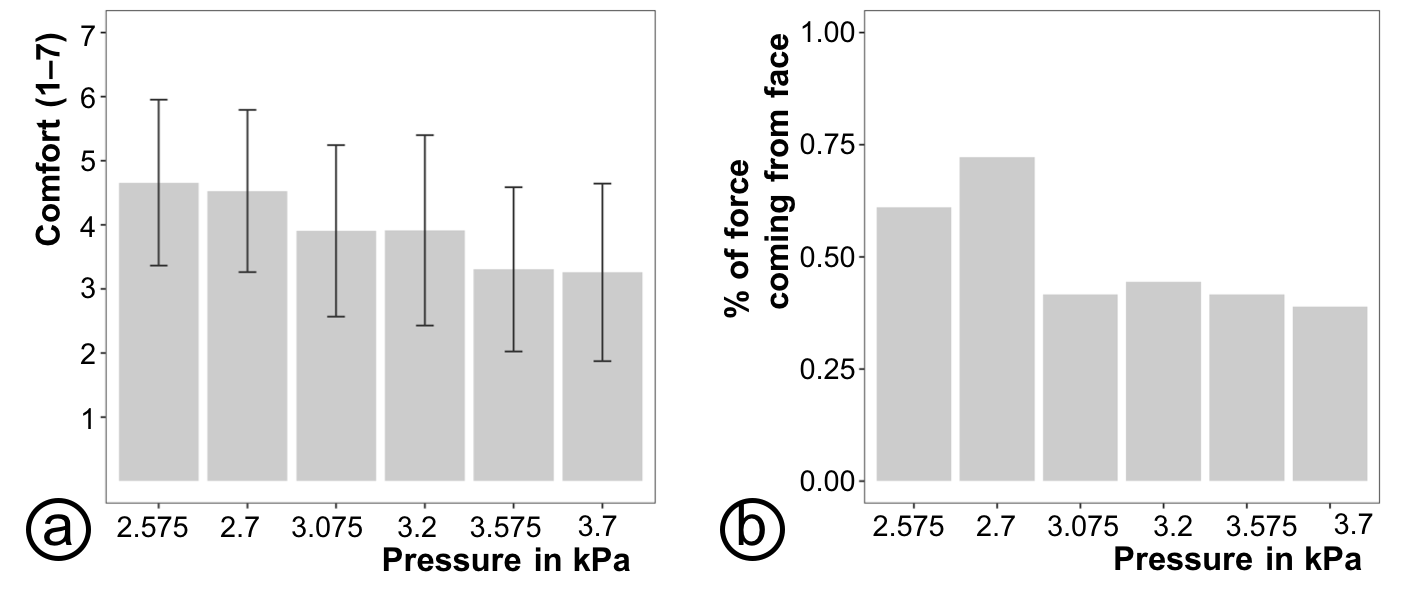
\includegraphics[width=1\linewidth]{figures/comfort}
        \end{tabular}
        \caption{(a) Comfort of each pressure (b) Judging the percentage of pressure on the face}
\label{fig:comfort}
    \end{center}
\end{figure}

\section{User Study 2: User Experience }
To survey the influences that FacePush can provide from the virtual world, we conducted a user study on the users of the boxing simulation. For this purpose, we immersed participants in a simplified study version of our boxing application. The participants cannot avoid being hit by the avatar. The avatar is displayed in front of the users and throws punches at the user consecutively. The level of realism and enjoyment are measured by their subjective ratings.

\subsection{Participants }
12 participants (7 females and 5 males, aged 21-25, mean age = 23.66) were recruited from our institution. Three of them had had no previous VR experience. Each participant received a small gratituity after completing our study.

\subsection{Experimental Design }
This experiment explores the effect of FacePush related to subjective ratings and head rotation. We vary the levels of FacePush as follows: 1) No-FacePush effect; the participants only wear the HMD mounted with FacePush but the FacePush device does not apply its effect. 2) FacePush with light pressure only; the intensity of each push was a constant of 2.7 kPa. 3) FacePush with heavy pressure only; the intensity of each push was a constant with 3.2 kPa. And, 4) FacePush with diverse pressure; FacePush exerts two different intensity stimuli (2.7 and 3.375 kPa) on the participants based on our results from the JND study. Each participant walks through four conditions and must assess the levels of realism and enjoyment of experiencing VR boxing.

To control the visual input across the four conditions, we display the animation of punches in accordance with a fixed order. The interval between two consecutive punches is 4 seconds long and each punch lasts approximately 0.5 seconds. The entire clip of animation for one condition runs for one minute. We asked the participants to wear earphones emitting pink noise as in the study 1.

\subsection{Procedures }
At the beginning of each trial, we asked the participants to maintain a standing pose and hold the Vive hand-held controllers in both hands so that they can fight against their opponents. After each condition, we asked participants to fill out a customized questionnaire to measure their experience of realism and enjoyment. The responses of questionnaire are on a 7-point Likert scale and allow for decimal responses. The order of conditions for each participant is determined by a 4x4 Latin square. Afterward, an open-ended interview to elicit general comments about the system is conducted. We also asked participants to rank their preferences of the four conditions according to their experience of realism and enjoyment respectively.

\subsection{Results }

\begin{figure}[h]
    \begin{center}
        \begin{tabular}{@{\hspace{0.1cm}}c}
        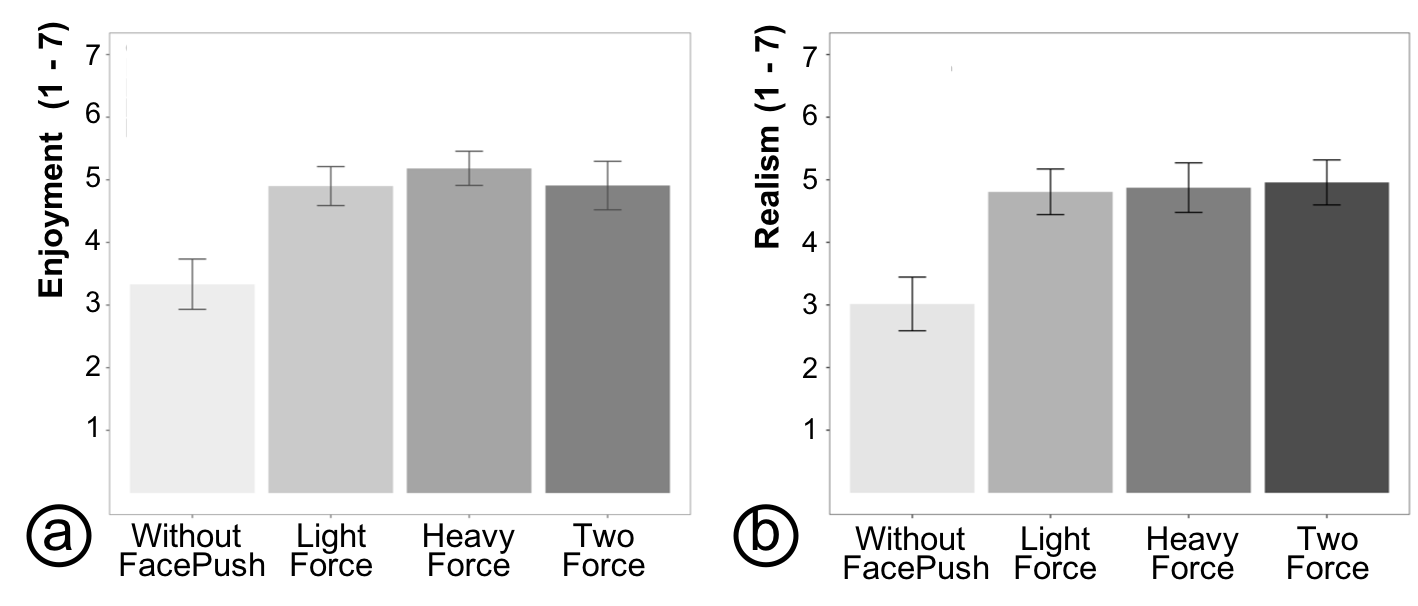
\includegraphics[width=1\linewidth]{figures/enjoymentrealism.png}
        \end{tabular}
        \caption{The subjective ratings for Enjoyment and Realism with regards to a virtual boxing application.}
        \label{fig:enjoymentrealism}
    \end{center}
\end{figure}

\subsubsection{Enjoyment}
Figure \ref{fig:enjoymentrealism} a shows the subjective ratings of enjoyment (The error-bar represents a 95\% of confidence interval). The level of No-FacePush received the lowest ratings (3.33, SD: 1.42). The ratings for the other three levels, light pressure (4.90, SD: 1.10), heavy pressure (5.18, SD: 0.965), and diverse pressure (4.91, SD: 1.37), are similar. The results of a one-way repeated measured ANOVA analysis indicates a significant difference in enjoyment ($F_{3, 33} = 22.894, p < .001$). We applied a pairwise test of means to examine the differences between level pairs. After Bonferroni correction, the level of No-FacePush is found to be significantly lower than the other three levels (light: $t_{11} = -5.585, p < .001$, heavy: $t_{11} = -5.457, p < .01$, diverse: $t_{11} = -7.021, p < .001$). The comparisons among light, heavy, and diverse levels showed no difference (light to heavy: $t_{11} = -1.982, p = 0.438$, light to diverse: $t_{11} = -0.039, p = 1$, heavy to diverse: $t_{11} = 1.104, p = 1$).

\subsubsection{Realism}
As shown in Figure \ref{fig:enjoymentrealism} b, the mean and 95\% confidence interval of subjective ratings of realism are presented. The condition of No-FacePush received the lowest rating (3.02, SD: 1.52); light pressure (4.81, SD: 1.29), heavy pressure (4.88, SD: 1.40), and diverse pressure (4.96, SD: 1.27). We conducted a one-way repeated measured ANOVA analysis and the violations to sphericity used Greenhouse-Geisser corrections to the degrees of freedom. The results indicate that the levels of FacePush show a significant difference in realism ($F_{3, 33} = 16.788, p < .001$). After Bonferroni correction, the pairwise test of means was performed and the result show that th No-FacePush level has a significant difference between light ($t_{11} = -4.579, p < .01$), heavy ($t_{11} = -4.381, p < .01$), and diverse levels ($t_{11} = -5.328, p < .01$). The comparison between light, heavy, and diverse levels showed no difference (light to heavy: $t_{11} = -0.628, p = 1$, light to diverse: $t_{11} = -0.625, p = 1$, heavy to diverse: $t_{11} = -0.279, p = 1$).

\subsection{Discussion }
Apart from these subjective ratings, we received user feedbacks from the interviews conducted afterward. In the interview, we asked participants to rank their preference of enjoyment and realism according to the four conditions they had experienced. Most of the participants rank the No-FacePush condition as the lowest and have a preference for the strong pressure or diverse pressure condition. This feedback corresponds to our results from inference statistics that levels of enjoyment and realism without FacePush are significantly lower than other conditions.

Users stated that, \textit{``I sometimes felt my glasses pressed while FacePush is pushing'' (P9)} and \textit{``I felt nausea during the boxing experience'' (P11)}. These uncomfortable outcomes may be caused by the distance shrinking from eyes to the lens of the HMD during pushing. This may cause the focus to change temporarily and cause nausea and blurred vision. However, we wish to stress that the participants did not explicitly report such an issue during the FacePush interaction. We think it is in part because the lens resets as soon as the short (and fast) feedback is finished during the boxing and diving applications. In the 360 video guidance trial, the continuous feedback may last longer, but the blurring effect may be ignored by users due to the only light pushes (thus short displacement) that are applied to the user's face for directional cues.

We consider that future research can address this by automating the focus adjustment via hardware solutions \cite{Konrad:2016:NOC:2858036.2858140,Optimizing.virtual.reality,Varifocal}, which exploited focus-tunable and multi-focus lenses to automatically adjust lens positions to reduce visual discomfort. Although their aim is to reduce the visual discomfort caused by vergence-accommodation conflict, the adjustment mechanism could be utilized to mitigate the lens displacement made by FacePush.In general, participants felt engaged with FacePush. For example, one participant stated that \textit{``The entire experience was very impressive, and the combination of punch feedback using FacePush was realistic.'' (P7)}. 

Our FacePush system provides only a part of the haptic feedback for a series of human sensations. Impacto \cite{Impacto} simulates boxing haptics through tactile feedback and impact movement. In future studies, FacePush's boxing experience can be enhanced with Impacto's mechanism, e.g., leading the normal force with a tactile feedback on the face. In the underwater swimming scenario, FacePush can be integrated with the thermal modules as per ThermoVR \cite{ThermoVR} to bring about sensations of coldness and distinctive current of water flowing simultaneously to enhance the user experience.

